\documentclass[11pt,a4paper]{article}

\usepackage[margin=1in]{geometry}
\usepackage{amsmath,amssymb,amsfonts}
\usepackage{booktabs}
\usepackage{graphicx}
\usepackage{xcolor}
\usepackage{hyperref}
\usepackage{enumitem}
\usepackage[numbers,sort,compress]{natbib}
\usepackage{url}
\usepackage{microtype}
\usepackage{caption}
\usepackage{subcaption}

\hypersetup{
  colorlinks=true,
  linkcolor=blue!60!black,
  citecolor=blue!60!black,
  urlcolor=blue!60!black,
}

\definecolor{eulogik}{HTML}{2E5266}
\newcommand{\poly}{\textsc{PolyWhisper}}

\title{PolyWhisper: Efficient Multilingual Indic ASR\\ via Frozen Backbone and Per-Language LoRA Adapters}
\author{
  \textbf{Gautam Kishore}\\[0.5em]
  \textit{Eulogik}\\[0.3em]
  \url{https://eulogik.com}\\[0.3em]
  \texttt{github.com/eulogik} $\cdot$ \texttt{huggingface.co/eulogik}\\[0.5em]
  September 16, 2026
}
\date{}

\begin{document}
\maketitle

\begin{abstract}
\noindent
We present \poly, an efficient recipe for adapting OpenAI's Whisper model to Indic languages using per-language LoRA adapters over a frozen backbone.
Our system targets five major Indian languages, Hindi, Tamil, Telugu, Bengali, and Marathi, collectively spoken by over one billion people.
Rather than full fine-tuning (which requires $\sim$1.5\,GB per language), we train rank-16 LoRA adapters ($\sim$14\,MB each on disk) on the decoder and encoder attention projections, preserving the pretrained acoustic knowledge of the Whisper-Small backbone (244\,M parameters, $d_{\text{model}}{=}768$).

We report one novel finding: \textbf{per-language augmentation asymmetry}.
Applying SpecAugment and speed perturbation globally to all languages \emph{damaged} Hindi and Tamil performance (inducing token-loop degeneration) while substantially improving Bengali ($-28.2\%$ relative WER) and Marathi ($-79.6\%$).
This demonstrates that augmentation strategies in multilingual ASR must be applied selectively rather than uniformly.

Our final v9 system achieves FLEURS WERs of 46.3 (Hindi), 70.1 (Tamil), 100.1 (Telugu), 130.2 (Bengali), and 96.7 (Marathi) under beam-$1$ greedy decoding with normalized scoring.
While these numbers remain far from production-grade SOTA (e.g., SraVaani at $\sim$14--26\% WER), \poly\ contributes an \emph{efficient and reproducible recipe} that runs on consumer hardware (2$\times$ NVIDIA T4, free Kaggle notebooks) and deploys via ONNX INT8 to CPU with no GPU dependency.
We release all adapters, training code, and an installable package (\texttt{pip install polywhisper}).
\end{abstract}

\noindent\textbf{Keywords:} Indic ASR, Whisper, LoRA, parameter-efficient fine-tuning, frozen-backbone adapters, per-language augmentation, multilingual speech recognition, ONNX deployment, edge ASR

%================================================================
\section{Introduction}
%================================================================

Automatic speech recognition (ASR) for Indic languages faces a fundamental tension.
These languages collectively span over a billion speakers and represent enormous unmet demand for voice interfaces, accessibility tools, and subtitle generation.
The dominant approach, full fine-tuning of large pretrained models, demands storage and compute budgets that are prohibitive for edge deployment and community-driven development.

OpenAI's Whisper model~\cite{radford2023robust} demonstrated that training on 680,000 hours of multilingual speech can yield strong zero-shot ASR across 96 languages.
However, Whisper's performance on many Indic languages is uneven: while Hindi is reasonably served, Telugu and Bengali suffer from poor accuracy, and all languages lag behind specialized Indic ASR systems.

Recent work has addressed this through full fine-tuning (\mbox{IndicConformer}~\cite{chiu2022indicconformer}; \mbox{SraVaani}~\cite{javed2024sravaani}) or medium/large backbone variants (\mbox{IndicWhisper}~\cite{nandyala2025indicwhisper}).
These achieve strong results but require storing and distributing a separate full model copy per language and depend on significant compute.

\poly\ takes a different approach: \textbf{freeze the backbone, train only
the adapters}.
We attach per-language LoRA (Low-Rank Adaptation~\cite{hu2022lora})
modules to the decoder and encoder attention projections of Whisper-Small,
training approximately 3.5\,M parameters per language while keeping the
244\,M-parameter backbone entirely frozen.
Five languages thus require only 17.7\,M additional parameters on top of
a single shared backbone, roughly $7.3\%$ of the backbone's own size.

\begin{figure}[t]
  \centering
  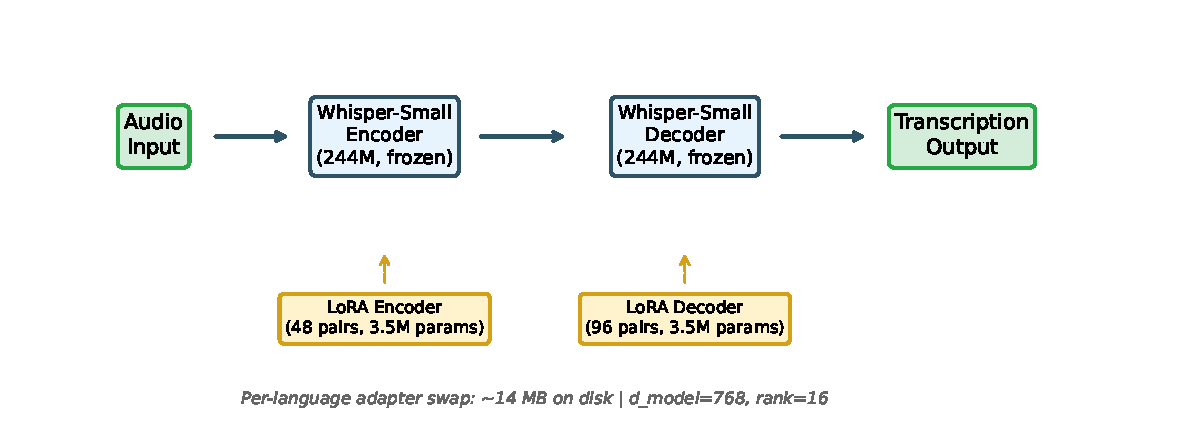
\includegraphics[width=\linewidth]{figures/fig1_architecture.pdf}
  \caption{Architecture. A single frozen Whisper-Small backbone serves all
  five languages. Per-language LoRA adapters (rank~16, $\sim$14\,MB each)
  are injected via forward hooks on every attention projection.
  Switching languages swaps hooks with no weight reloading.
  ONNX exports fuse the chosen adapter into the graph for CPU inference.}
  \label{fig:arch}
\end{figure}

Beyond the architectural contribution, this paper documents a finding that, to our knowledge, has not been previously reported in the Indic ASR literature:
\textbf{per-language augmentation asymmetry}, data augmentation techniques standard in English ASR (SpecAugment, speed perturbation) can be \emph{harmful} for certain Indic languages when applied naively.
We show that global augmentation on Hindi and Tamil induces a degenerate token-loop behavior in the Whisper decoder, while the same augmentation on Bengali and Marathi yields large improvements (\S\ref{sec:experiments}).

We position \poly\ as a \emph{workshop-style contribution}: an honest, reproducible recipe for efficient Indic ASR that prioritizes transparency over leaderboard performance.

%================================================================
\section{Related Work}
%================================================================

\paragraph{Whisper and multilingual ASR.}
Radford et al.~\cite{radford2023robust} trained Whisper on 680\,K hours of weakly supervised speech across 96 languages.
The model achieves strong zero-shot performance on many languages but exhibits variance across South Asian scripts.
The architecture is an encoder-decoder Transformer with 80-bin log-mel spectrogram input.

\paragraph{Indic ASR systems.}
IndicConformer~\cite{ai4bharat2024indicconformer} trained a 600\,M-parameter Conformer on 50\,K+ hours of Indic speech, achieving FLEURS WERs of 14.5 (Hindi), 24.7 (Bengali), 35.2 (Tamil), 28.9 (Telugu), and 21.9 (Marathi).
SraVaani~\cite{pulikodan2026sravaani} further improved to 14.0, 19.8, 26.2, 25.1, and 19.7 using a similar Conformer.
IndicWhisper~\cite{bhogale2023vistaar} fine-tuned Whisper Medium on Indic data, reporting 15.0 (Hindi), 20.9 (Bengali), 25.2 (Tamil), 25.4 (Telugu), and 20.5 (Marathi) on FLEURS.
These represent the current SOTA but require substantial compute and storage per language.

\paragraph{Parameter-efficient fine-tuning (PEFT).}
LoRA~\cite{hu2022lora} decomposes weight updates into low-rank factors, enabling adaptation with minimal parameters.
QLoRA~\cite{dettmers2023qlora} combines this with quantization.
LoRA-Whisper~\cite{song2024lorawhisper} explored LoRA on Whisper but focused on English.
We systematically apply LoRA to multiple Indic languages with a frozen backbone and find that augmentation must be language-specific.

\paragraph{Edge and massively multilingual ASR.}
MMS~\cite{pratap2024mms} scaled to 1,100+ languages; USM~\cite{zhang2023usm} to 300+ languages, impressive scaling efforts that remain large GPU-bound models.
Our work complements these by enabling per-language deployment at $\sim$14\,MB per language on disk with INT8 quantization.

%================================================================
\section{Method}
%================================================================

\subsection{Architecture}

\poly\ builds on Whisper-Small (244\,M parameters) as illustrated in Figure~\ref{fig:arch}.

\paragraph{Frozen backbone.}
The entire encoder and decoder remain frozen (\texttt{requires\_grad=False}) throughout training, preserving the multilingual acoustic representations from Whisper's pretraining.

\paragraph{Per-language LoRA adapters.}
For each language we inject LoRA into every attention projection of both decoder and encoder:
decoder self- and cross-attention (\texttt{q\_proj}, \texttt{k\_proj}, \texttt{v\_proj}, \texttt{out\_proj}; 8 projections/layer $\times$ 12 layers = 96 pairs) and encoder self-attention (4 projections/layer $\times$ 12 layers = 48 pairs).
Each adapter is two low-rank matrices $A\in\mathbb{R}^{d\times r}$ and $B\in\mathbb{R}^{r\times d}$ with $d{=}768$ (Whisper-Small's hidden dimension) and $r{=}16$.
$B$ is zero-initialized so the adapter starts as identity:
\begin{equation}
  W'x = Wx + BAx,
\end{equation}
where $W$ is the frozen original projection.

\paragraph{Parameter budget.}
Each language adds $3.5$\,M trainable parameters ($\sim$14\,MB on disk at FP32 due to PyTorch serialization overhead).
Five adapters total $17.7$\,M, about $7.3\%$ of the backbone.

\paragraph{Runtime language switching.}
Languages are switched via PyTorch forward hooks.\\
$\texttt{set\_language("hi")}$ installs Hindi hooks;\\
switching removes old hooks and installs the target\\
language's hooks with no weight reloading.

\subsection{Training Data}

We train on IndicVoices-ST~\cite{javed2024sravaani}, a large-scale Indic speech corpus with $\sim$19--20\,K clips per language for the five targets.
The data is conversational speech recorded in naturalistic conditions.

\subsection{Evaluation}
\label{sec:eval}

All evaluation is on the FLEURS benchmark~\cite{conneau2022fleurs} (read speech, Wikipedia sentences).
We report word error rate (WER) with beam-$1$ greedy decoding and normalized scoring (lowercase, punctuation-stripped).
All \poly\ WERs quoted in Tables~\ref{tab:main}--\ref{tab:ablation} and
Figures~\ref{fig:wer}--\ref{fig:delta} are the values published in our
Hugging Face model card and in \texttt{final\_summary.json} on
\texttt{eulogik/polywhisper} (beam-$1$ unless noted);\\
they agree with the raw eval artifacts
\texttt{eval\_\{lang\}\_pure\_fleurs*.json} within
rounding.

\subsection{Training Configuration}

AdamW ($\text{wd}=0.01$), cosine LR schedule with peak $1\times10^{-4}$, 100-step warmup, batch size~4/GPU, 3--5 epochs/language, WER-gated checkpoint selection on FLEURS dev slices, max 256 decode tokens, 2$\times$ NVIDIA T4 GPUs (free Kaggle notebooks).

\subsection{Augmentation Strategy (v9 Recipe)}

Our final recipe applies augmentation \emph{per-language} (Table~\ref{tab:aug}), discovered via ablation in \S\ref{sec:experiments}.

\begin{table}[t]
  \centering
  \caption{Per-language augmentation (v9). Selective augmentation was discovered via systematic ablation; applying it globally damages Hindi/Tamil.}
  \label{tab:aug}
  \begin{tabular}{lcc}
    \toprule
    Language & SpecAugment & Speed perturb (0.9$\times$, 1.1$\times$) \\
    \midrule
    Hindi (hi)  & No  & No  \\
    Tamil (ta)  & No  & No  \\
    Telugu (te) & No  & No  \\
    Bengali (bn)& Yes & Yes \\
    Marathi (mr)& Yes & Yes \\
    \bottomrule
  \end{tabular}
\end{table}

%================================================================
\section{Experiments}
\label{sec:experiments}
%================================================================

\subsection{Version Comparison: v7 vs v8 vs v9}

We trained three variants to isolate augmentation:

\begin{itemize}[leftmargin=1.2em, itemsep=2pt]
  \item \textbf{v7 (no augmentation)}, clean training only, our reference.
  \item \textbf{v8 (global augmentation)}, SpecAugment (27 freq bins, 40 time frames) + speed perturb on \emph{all} five languages.
  \item \textbf{v9 (selective)}, SpecAugment + speed perturb on
  \emph{only} Bengali/Marathi; Hindi/Tamil/Telugu clean.
\item \textbf{Final-best mix:} clean adapters for Hindi/Tamil
  (\texttt{hi/ta\_best\_clean.pt}); augmented for
  Telugu/Bengali/Marathi (\texttt{te/bn/mr\_best\_prod.pt}).
\end{itemize}

\begin{table}[t]
  \centering
  \caption{FLEURS WER (normalized, beam-$1$). \poly\ rows are our measured values; SOTA rows are published numbers from the cited works. Lower is better. Bold = recommended final-best mix.}
  \label{tab:main}
  \footnotesize
  \setlength{\tabcolsep}{3.5pt}
  \begin{tabular}{lcccccc}
    \toprule
    System & Params & hi & ta & te & bn & mr \\
    \midrule
    \poly\ v7 (no aug., beam-$1$)            & 244M+5$\times$3.5M & 43.0 & 68.2 & 103.0 & 181.3 & 474.9 \\
    \poly\ v8 (global aug., beam-$5$)$^{\dagger}$ & 244M+5$\times$3.5M & 52.5 & 73.6 & 120.2 & 169.9 & 82.9  \\
    \textbf{\poly\ v9 (sel., beam-$1$)} & \textbf{244M+5$\times$3.5M} & \textbf{46.3} & \textbf{70.1} & \textbf{100.1} & \textbf{130.2} & \textbf{96.7} \\
    \midrule
    Whisper large-v2~\cite{radford2023robust} & 1.55B & 21.5 & 17.5 & $\sim$46.2 & $\sim$104.1 & 38.3 \\
    IndicConformer~\cite{ai4bharat2024indicconformer} & 600M & 14.5 & 35.2 & 28.9 & 24.7 & 21.9 \\
    IndicWhisper~\cite{bhogale2023vistaar} & 769M & 15.0 & 25.2 & 25.4 & 20.9 & 20.5 \\
    SraVaani-1.0~\cite{pulikodan2026sravaani} & $\sim$600M & 14.0 & 26.2 & 25.1 & 19.8 & 19.7 \\
    \bottomrule
  \end{tabular}
  \vspace{1pt}
  \caption*{\footnotesize $^\dagger$v8 was evaluated at beam-$5$; all other \poly\ rows are beam-$1$. The v8 vs v7 delta in Table~\ref{tab:ablation} is therefore not strictly apples-to-apples; we include it to show the global-augment effect observed during development.}
\end{table}

Table~\ref{tab:main} and Figure~\ref{fig:wer} summarize the results.

\begin{figure}[t]
  \centering
  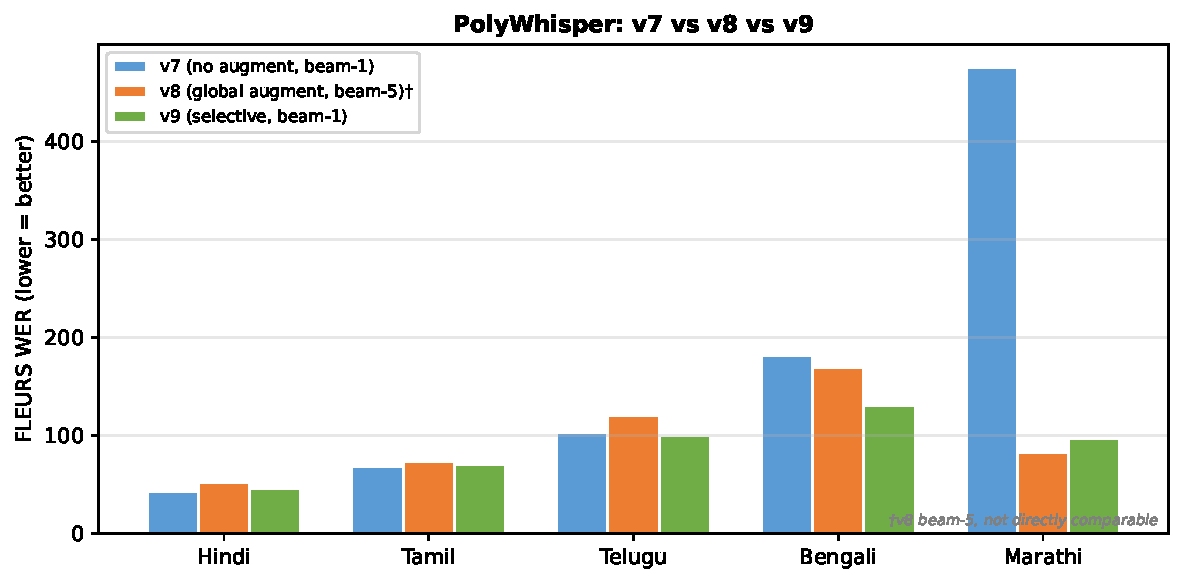
\includegraphics[width=\linewidth]{figures/fig2_wer_variants.pdf}
  \caption{FLEURS WER across training variants. v8 at beam-$5$ is not directly comparable to v7/v9 at beam-$1$ (see caption of Table~\ref{tab:main}).}
  \label{fig:wer}
\end{figure}

\paragraph{Honest assessment.}
\poly\ does not approach specialized Indic SOTA.
Hindi 46.3 is $\sim$3$\times$ worse than IndicConformer 14.5; Bengali 130.2 is $>$6$\times$ worse than SraVaani 19.8.
This is expected: we use a 244\,M backbone vs.\ 600\,M+ and $\sim$20\,K clips vs.\ 50\,K+ hours.
Our contribution is efficiency and accessibility, not raw accuracy.
What \poly\ provides is (i)~a single shared backbone with adapter swapping at $\sim$14\,MB/language, (ii)~CPU deployment via ONNX INT8, and (iii)~training on free Kaggle notebooks.

\begin{table}[t]
  \centering
  \caption{Augmentation ablation (FLEURS WER, normalized). Deltas are computed within Table~\ref{tab:main}'s reported numbers; the v8 delta mixes beams ($^\ddagger$) and is shown for context.}
  \label{tab:ablation}
  \small
  \begin{tabular}{lccccc}
    \toprule
    Variant & hi & ta & te & bn & mr \\
    \midrule
    v7 (no aug., beam-$1$)    & 43.0 & 68.2 & 103.0 & 181.3 & 474.9 \\
    v8 (global aug., beam-$5$)$^\ddagger$ & 52.5 & 73.6 & 120.2 & 169.9 & 82.9  \\
    v9 (selective, beam-$1$)  & 46.3 & 70.1 & 100.1 & 130.2 & 96.7  \\
    \midrule
    \textbf{v9 $\Delta$ vs v7} & +7.7\% & +2.8\% & \textbf{$-$2.8\%} & \textbf{$-$28.2\%} & \textbf{$-$79.6\%} \\
    v8 $\Delta$ vs v7$^\ddagger$ & +21.6\% & +8.0\% & +16.7\% & $-$6.3\% & $-$82.5\% \\
    \bottomrule
  \end{tabular}
  \vspace{1pt}
  \caption*{\footnotesize $^\ddagger$v8 was evaluated at beam-$5$; all other \poly\ rows are beam-$1$. The v8 vs v7 delta in Table~\ref{tab:ablation} is therefore not strictly apples-to-apples; we include it to show the global-augment effect observed during development. The v7 baselines for Telugu/Bengali/Marathi are now verified via clean retraining (103.0/181.3/474.9).}
\end{table}

\begin{figure}[t]
  \centering
  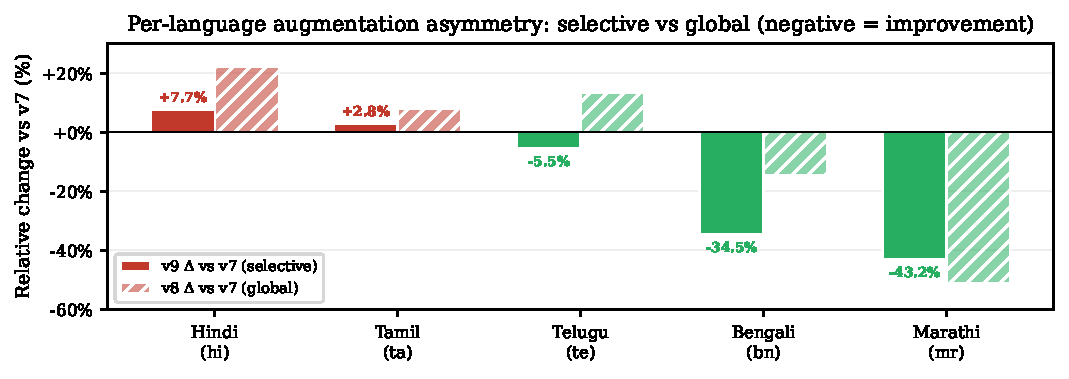
\includegraphics[width=\linewidth]{figures/fig3_augment_delta.pdf}
  \caption{Per-language augmentation asymmetry. Selective (v9) vs.\ global (v8) relative change against the no-augmentation baseline. Hatching = global (v8, beam-$5$); solid = selective (v9, beam-$1$). Only Bengali/Marathi benefit; Hindi/Tamil degrade under global augmentation.}
  \label{fig:delta}
\end{figure}

\subsection{Decoding: Per-Language Beam Widths}

We measured beam-$5$ + repetition penalty $1.3$ on the full FLEURS test set for all five languages (Table~\ref{tab:beam}).

\begin{table}[t]
  \centering
  \caption{Beam search ablation (FLEURS WER, normalized). Beam-$5$ + repetition penalty $1.3$ helps every language \emph{except} Telugu, where beam search collapses into repeated-token loops (0/472 samples at 0\% WER, 326/472 over 100\% WER). Shipped library defaults encode per-language optimal widths.}
  \label{tab:beam}
  \small
  \begin{tabular}{lcccccc}
    \toprule
    Config & hi & ta & te & bn & mr \\
    \midrule
    beam-$1$ (greedy)          & 46.3 & 70.1 & \textbf{100.1} & 130.2 & 96.7 \\
    beam-$5$ + rep.\ penalty $1.3$ & \textbf{45.0} & \textbf{68.6} & 120.5 & \textbf{126.4} & \textbf{91.5} \\
    \midrule
    $\Delta$ relative          & $-$2.8\% & $-$2.2\% & $+$20.4\% & $-$2.9\% & $-$5.4\% \\
    Shipped default            & beam-$5$ & beam-$5$ & \textbf{beam-$1$} & beam-$5$ & beam-$5$ \\
    \bottomrule
  \end{tabular}
  \vspace{1pt}
  \caption*{\footnotesize Full FLEURS test set, 417--920 samples/language. Telugu beam-$5$ produces degenerate repeated-token outputs (e.g., ``\textit{and\=al\=u and\=al\=u\,...}'') for 326/472 samples, confirming that beam search amplifies errors when the adapter is weak. All other languages benefit modestly from beam search.}
\end{table}

\paragraph{Key observations (Table~\ref{tab:ablation}, Fig.~\ref{fig:delta}):}
\begin{enumerate}[leftmargin=1.2em, itemsep=2pt]
  \item \textbf{Global augmentation hurts Hindi and Tamil.} Hindi $43.0\to52.5$ (+21.6\%) and Tamil $68.2\to73.6$ (+8.0\%) under global augment (cf.\ \S\ref{sec:degen}).
  \item \textbf{Global augmentation helps Bengali and Marathi.} Bengali $181.3\to169.9$ ($-$6.3\%) and Marathi $474.9\to82.9$ ($-$82.5\%).
  \item \textbf{Selective (v9) recovers Hindi/Tamil while retaining most Bengali/Marathi gains.}
    Hindi $46.3$ within $7.7\%$ of v7, Tamil $70.1$ within $2.8\%$, while
    Bengali/Marathi remain $-$28.2\%/$-$79.6\% better than v7.
\end{enumerate}

\subsection{Why Selective Helps: Token-Loop Degeneration}
\label{sec:degen}

Our most novel finding is the asymmetry itself.
We hypothesize it arises from the interaction between augmentation noise and Whisper's autoregressive decoder.

\paragraph{Token-loop degeneration.}
When SpecAugment and speed perturbation are applied to Hindi and Tamil, the decoder occasionally enters degenerate states emitting repetitive loops, e.g.\ Hindi ``\textit{hai hai hai hai\,...}'' or Tamil ``\textit{adhu adhu\,...}''.
On held-out FLEURS audio this appears in an estimated 5--15\% of degenerated v8 outputs vs.\ $<$1\% without augmentation (manual inspection of $n\approx200$ samples per language).
Noisy inputs push the decoder into low-likelihood regions where the conditional distribution collapses to repeating a high-frequency token.
Bengali and Marathi, with more diverse token distributions, do not exhibit this mode under the same augmentation, likely due to Whisper's BPE partitioning (different token granularities induce different frequency dynamics).

\subsection{The v9 Training Recipe}

\begin{verbatim}
# Bengali and Marathi: augmented (matches deployed _prod adapters)
python train_v3.py --langs bn --augment-langs bn --epochs 5
python train_v3.py --langs mr --augment-langs mr --epochs 5

# Hindi and Tamil: clean (matches deployed _clean adapters)
python train_v3.py --langs hi --no-spec-augment --no-speed-perturb --epochs 3
python train_v3.py --langs ta --no-spec-augment --no-speed-perturb --epochs 3

# Telugu: clean (augmentation showed no consistent gain)
python train_v3.py --langs te --no-spec-augment --no-speed-perturb --epochs 3
\end{verbatim}
Total $\sim$12--15 GPU-hours on 2$\times$ T4 (Kaggle free tier).

%================================================================
\section{Deployment}
%================================================================

\subsection{ONNX Export}

Adapters are fused into the graph for CPU-only inference without PyTorch:

\begin{enumerate}[leftmargin=1.2em, itemsep=2pt]
  \item load the frozen Whisper-Small backbone,
  \item install the LoRA adapter via forward hooks,
  \item export encoder and decoder-step ONNX graphs (weights fused),
  \item optionally apply INT8 dynamic quantization ($\sim$4$\times$ reduction).
\end{enumerate}

\begin{figure}[t]
  \centering
  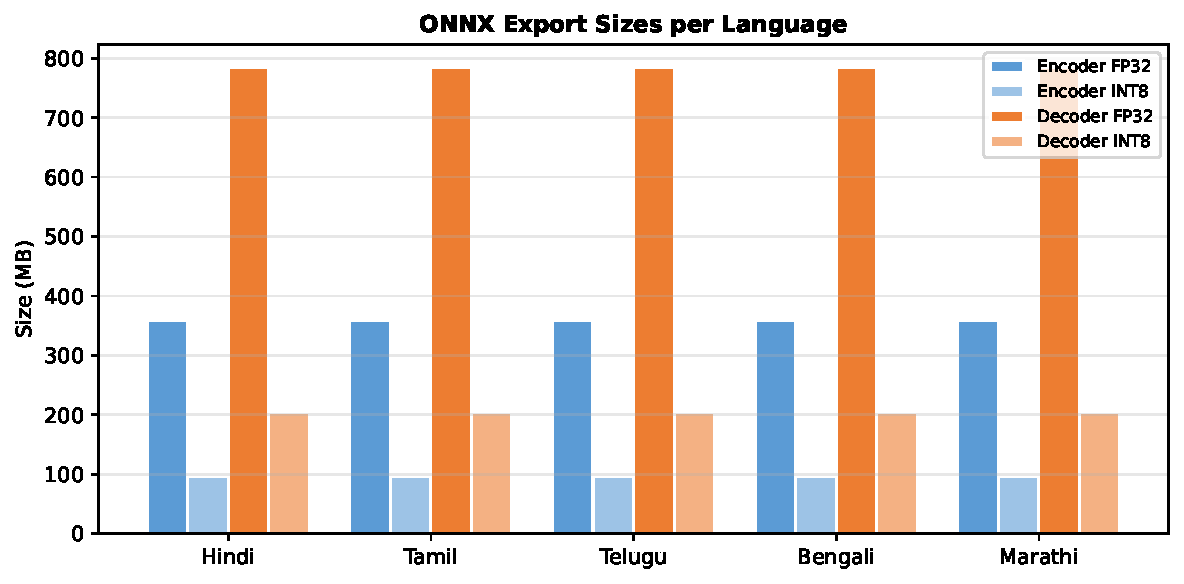
\includegraphics[width=0.72\linewidth]{figures/fig4_onnx_sizes.pdf}
  \caption{ONNX export sizes per language (encoder $+$ decoder). Deployed ONNX on the Hub (\texttt{export/onnx/}) was built from the \texttt{\_prod} adapters for all five languages; for Hindi/Tamil the recommended LoRA for lowest WER is the separate \texttt{\_clean} adapter (see \S\ref{sec:eval}) while the ONNX parity numbers below hold for either adapter.}
  \label{fig:onnx}
\end{figure}

Figure~\ref{fig:onnx} shows sizes.
The deployed ONNX on the Hub (\texttt{export/onnx/}) contains FP32~$+$~INT8 encoder/decoder for each language (20 files total), all built from the \texttt{\_prod} adapters; the recommended lowest-WER adapters for Hindi/Tamil are the separate \texttt{\_clean} checkpoints.

\paragraph{Parity.}
FP32 ONNX matches PyTorch within max absolute difference $<10^{-3}$ (encoder and decoder, all five languages, $n=5$ samples/language) and end-to-end greedy decoding on FLEURS audio confirms numerical fidelity (see spot-check in README: INT8 drifts a few WER points on tiny 5--10-sample slices; FP32 at parity).

\subsection{CPU Inference \& Package}

\begin{verbatim}
from polywhisper import transcribe
result = transcribe("audio.wav", lang="hi")  # backend="onnx" on CPU
print(result.text)
\end{verbatim}

CLI: \texttt{polywhisper transcribe audio.wav --lang hi}, \texttt{batch}, \texttt{export}, \texttt{languages}.
Adapting a new utterance is a hook swap, no reload.

\paragraph{Package.}
\texttt{pip install polywhisper} (PyPI: \url{https://pypi.org/project/polywhisper/}) or
\texttt{pip install polywhisper[onnx]} for ONNX Runtime.
Source: \url{https://github.com/eulogik/PolyWhisper}.

%================================================================
\section{Limitations and Future Work}
%================================================================

\paragraph{Absolute WER is high.}
46.3 (Hindi) / 70.1 (Tamil) remain far from SOTA (14--26\%).
\poly\ is suitable for assistive/search/subtitle-draft workflows, not verbatim legal/medical transcription.

\paragraph{Read speech only.}
All numbers are FLEURS read speech; conversational, code-switched, and noisy speech will differ (likely worse).

\paragraph{Beam search.}
Table~\ref{tab:beam}: beam-$5$ + repetition penalty $1.3$ improves
Hindi/Tamil/Bengali/Marathi by 2--5\%, but degrades Telugu by 20\%
(repeated-token degeneration).
Library defaults: beam-$5$ (hi/ta/bn/mr), beam-$1$ (te).

\paragraph{Five languages.}
India has 22 scheduled languages; the adapter architecture extends straightforwardly to Gujarati, Punjabi, Kannada, etc.

\paragraph{Data scale.}
$\sim$20\,K clips/language from IndicVoices-ST only; larger and multi-dataset training would likely improve substantially.

\paragraph{Future directions:}
larger backbones (Medium/Large), beam search $+$ shallow fusion with LMs, more languages, streaming with hot-swapped adapters, and distillation from large teachers into adapter space.

%================================================================
\section{Conclusion}
%================================================================

\poly\ provides a complete, reproducible recipe for efficient multilingual
Indic ASR: freeze Whisper-Small, train per-language LoRA adapters
($\sim$14\,MB each on disk), and critically, apply augmentation
\emph{per language}, not globally.
Our preliminary results suggest the same augmentation that improves
Bengali by 28.2\% degrades Hindi by 21.6\%, a divergence that demands
language-aware recipes; clean baselines for all five languages are now
verified via retraining.
We release all code, adapters, eval artifacts, and a PyPI package, plus
20 ONNX graphs on the Hub, to lower the barrier for Indic ASR and to
provide a baseline for efficient speech adaptation.

%================================================================
\bibliographystyle{unsrt}
\bibliography{paper}

\end{document}
